\section{Metalle}
Typische Eigenschaften: gute elektrische und Wärme-Leitfähigkeit, Duktilität, Glanz

\subsection{Kristallite und Gefüge}
Reales Metall ist ein Gefüge aus eine Vielzahl unregelmässig angeordneter Kristalle (polykristallin). Die Körner beeinflussen die Eigenschaften.

\subsection{Elektronengas-Modell}
Metallkationen bilden ein Gitter, die VE sind delokalisiert (frei beweglich), weil Metalle kleine Rumpfladung haben. 

\subsection{Metallische Bindung}
ungerichtete elektrostatische Anziehung zwischen Metallkationen und $e^-$-Gas. Sind stärker, je mehr Valenzelektronen ein Metallatom aufweist.

\subsection{Duktilität}
Reine Metalle sind relativ duktil, weil dichtest gepackte Schichten gut gegeneinander beweglich sind. Duktilität ist abhängig von der Zahl der Gleitebenen (d.h. Gittertyp, Korngrösse), der Stärke der metall. Bindung und der Gitterfehler. 

\subsection{Legierungen}
Stoffe, die aus zwei oder mehr Elementen bestehen und metallische Eigenschaften aufweisen.

\subsubsection{Eigenschaften}
\begin{itemize}
	\item Härte: Legierungen sind härter als reine Metalle. Ursache: Fremdatome behindern Gleitebenen.
	\item El. Leitfähigkeit: schlechtere leitend als Metalle. Ursache: Fremdatome behindern $e^-$-Fluss.
	\item Korrosionsbeständigkeit: meist korrosionsbeständiger als Metalle.
\end{itemize}

\begin{figure}[htbp]
	\centering
	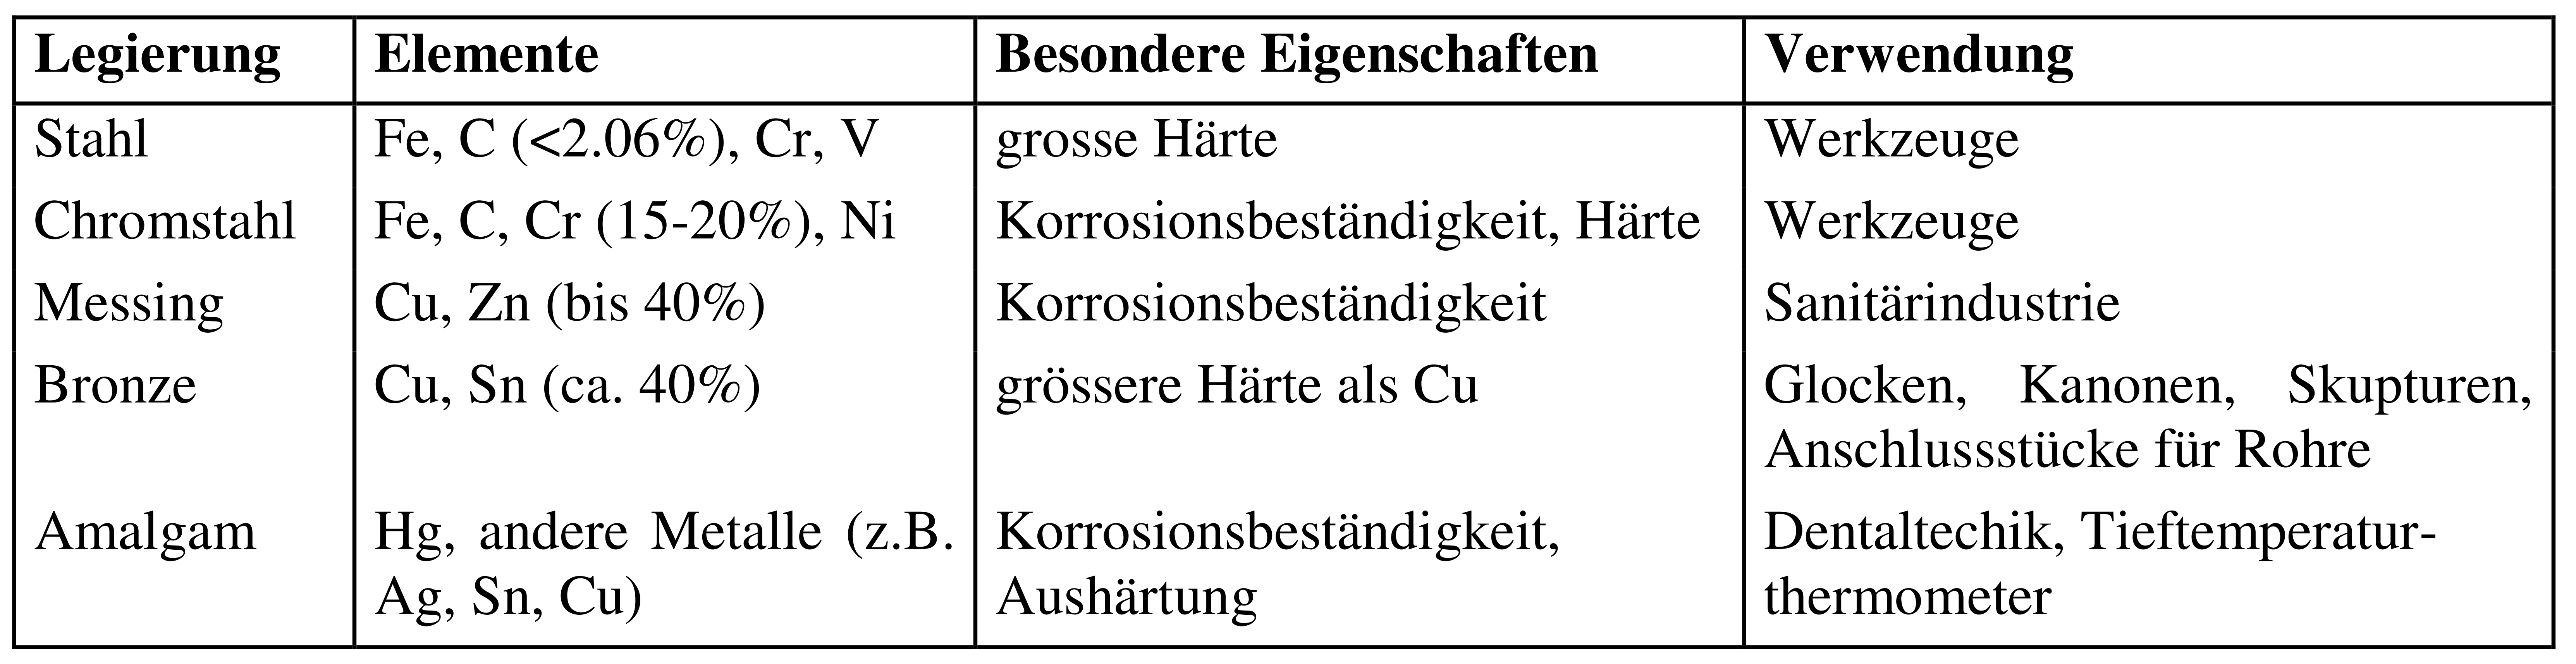
\includegraphics[width=1\linewidth]{images/3_Legierungen.png}
\end{figure}

\subsubsection{Substitutionslegierungen}
Gewisse Basismetallatome sind durch Fremadatome ersetzt. Bilden sich, wenn die Fremdatome ähnliche Atomradien und Bindungscharakteristiken wie die Metallatome haben.

\begin{figure}[htbp]
	\begin{subfigure}{0.32\linewidth}
		\centering
		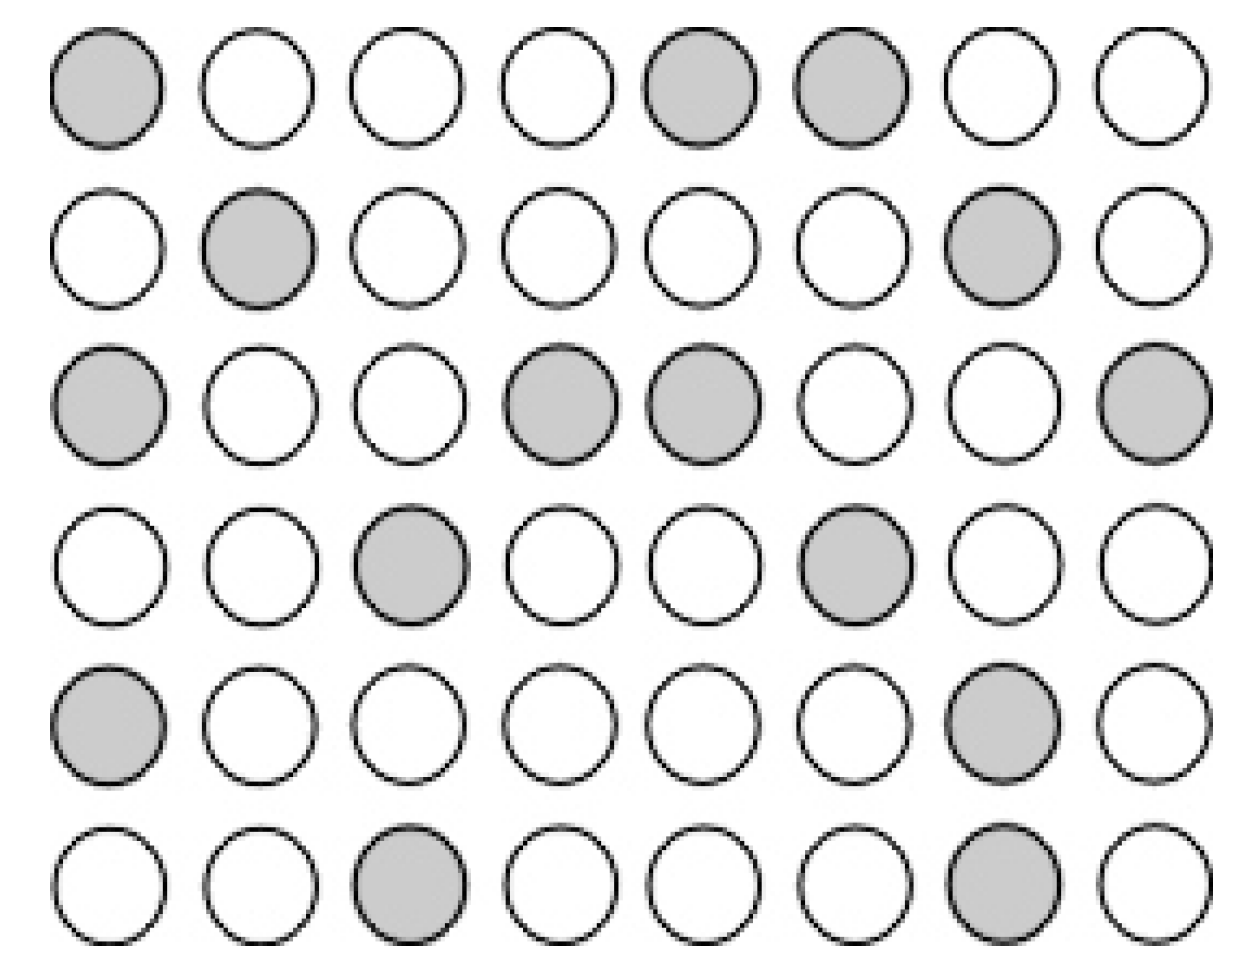
\includegraphics[width=0.75\linewidth]{images/3_Subst_1.png}
		\caption{Kristallit ungeregelt subtituiert}
	\end{subfigure}
	\begin{subfigure}{0.32\linewidth}
		\centering
		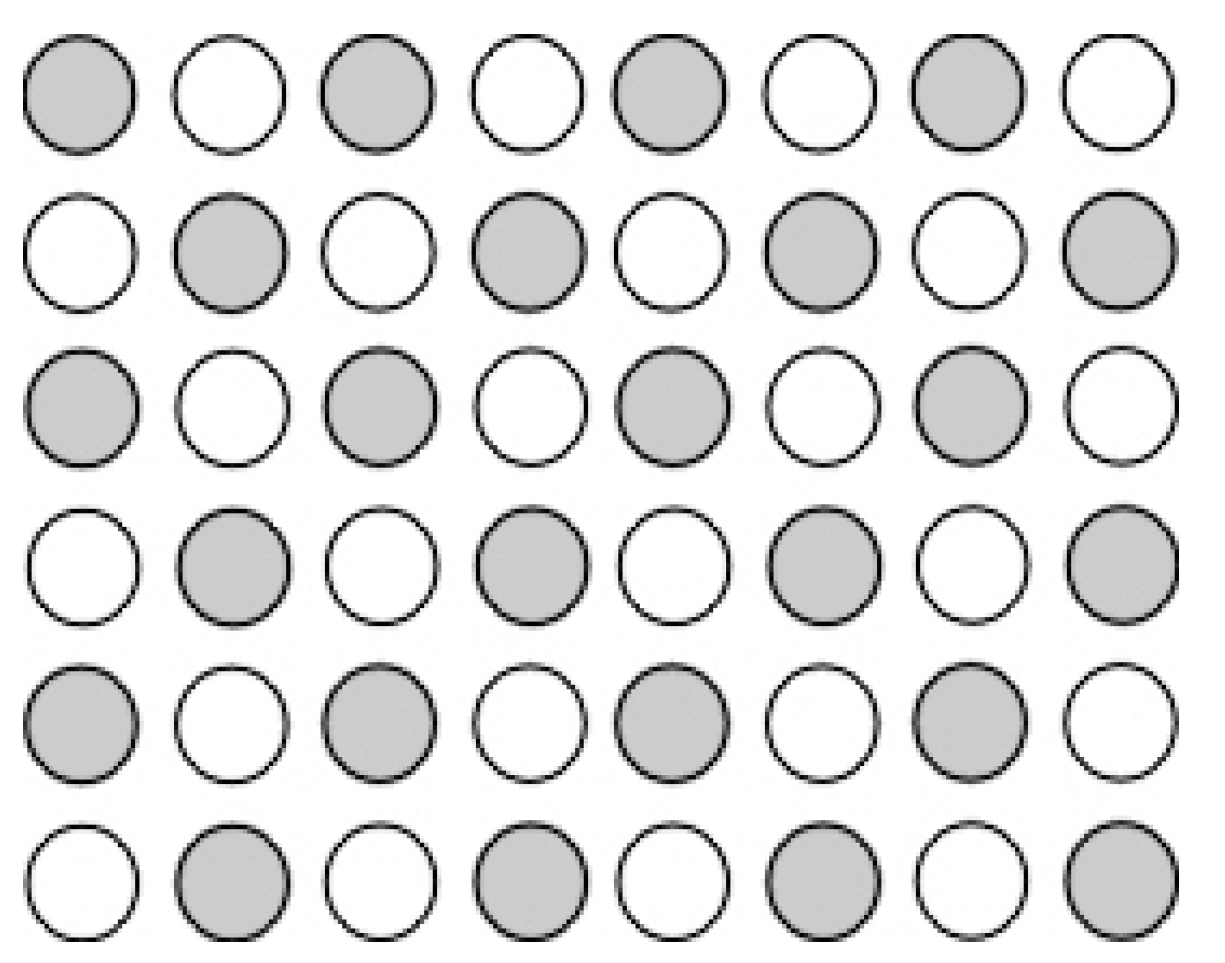
\includegraphics[width=0.75\linewidth]{images/3_Subst_2.png}
		\caption{Kristallit geregelt substituiert}
	\end{subfigure}
	\begin{subfigure}{0.32\linewidth}
		\centering
		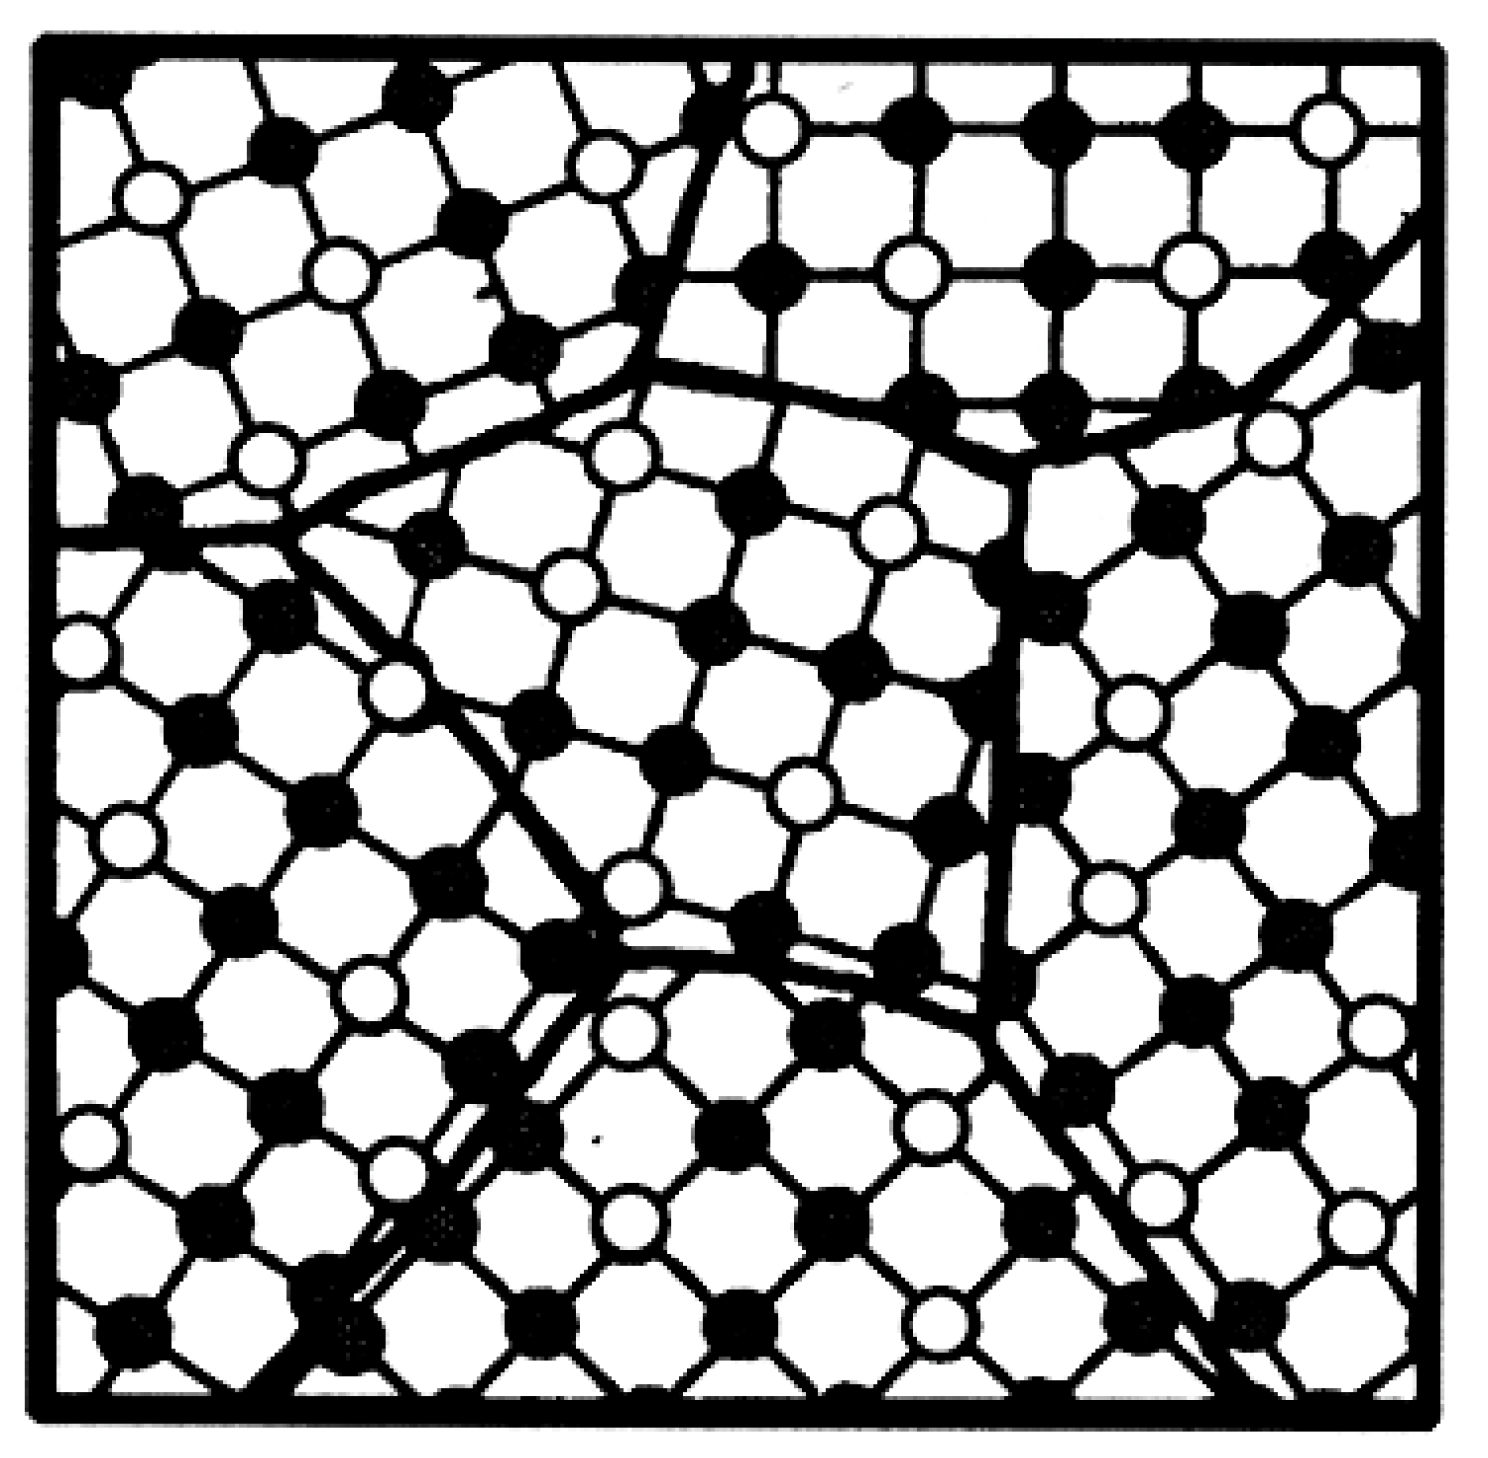
\includegraphics[width=0.75\linewidth]{images/3_Subst_3.png}
		\caption{Aufbau einer ungeregelten Substitutionslegierung}
	\end{subfigure}
\end{figure}

\subsubsection{Einlagerungslegierungen}
Fremdatome besetzen Oktaeder- oder Tetraederlücken der Metallatome. Entstehen wenn eine Atomart viel kleiner ist als die Metallatome

\begin{figure}[htbp]
	\begin{subfigure}{0.32\linewidth}
		\centering
		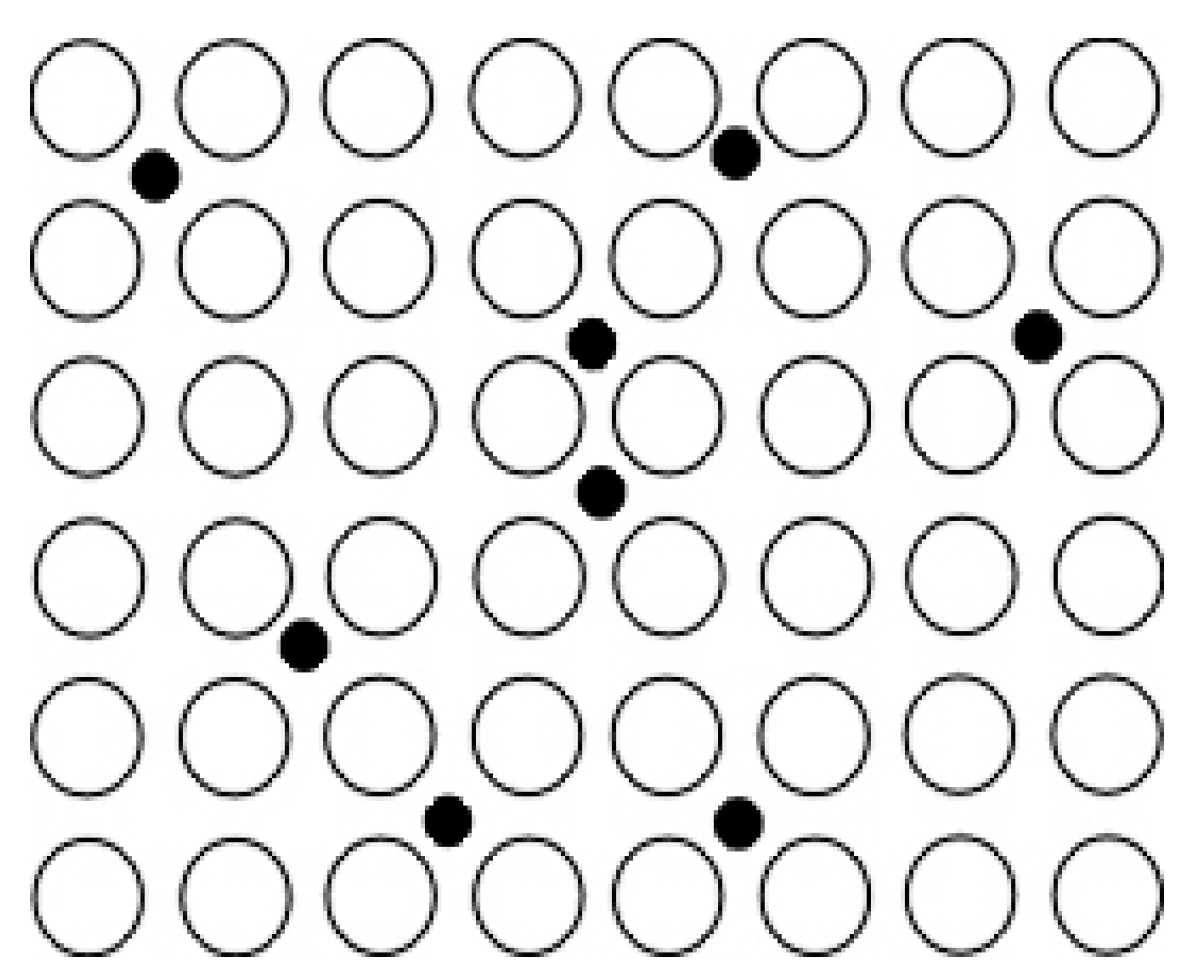
\includegraphics[width=0.75\linewidth]{images/3_Ein_1.png}
		\caption{Kristallit ungeregelt eingelagert}
	\end{subfigure}
	\begin{subfigure}{0.32\linewidth}
		\centering
		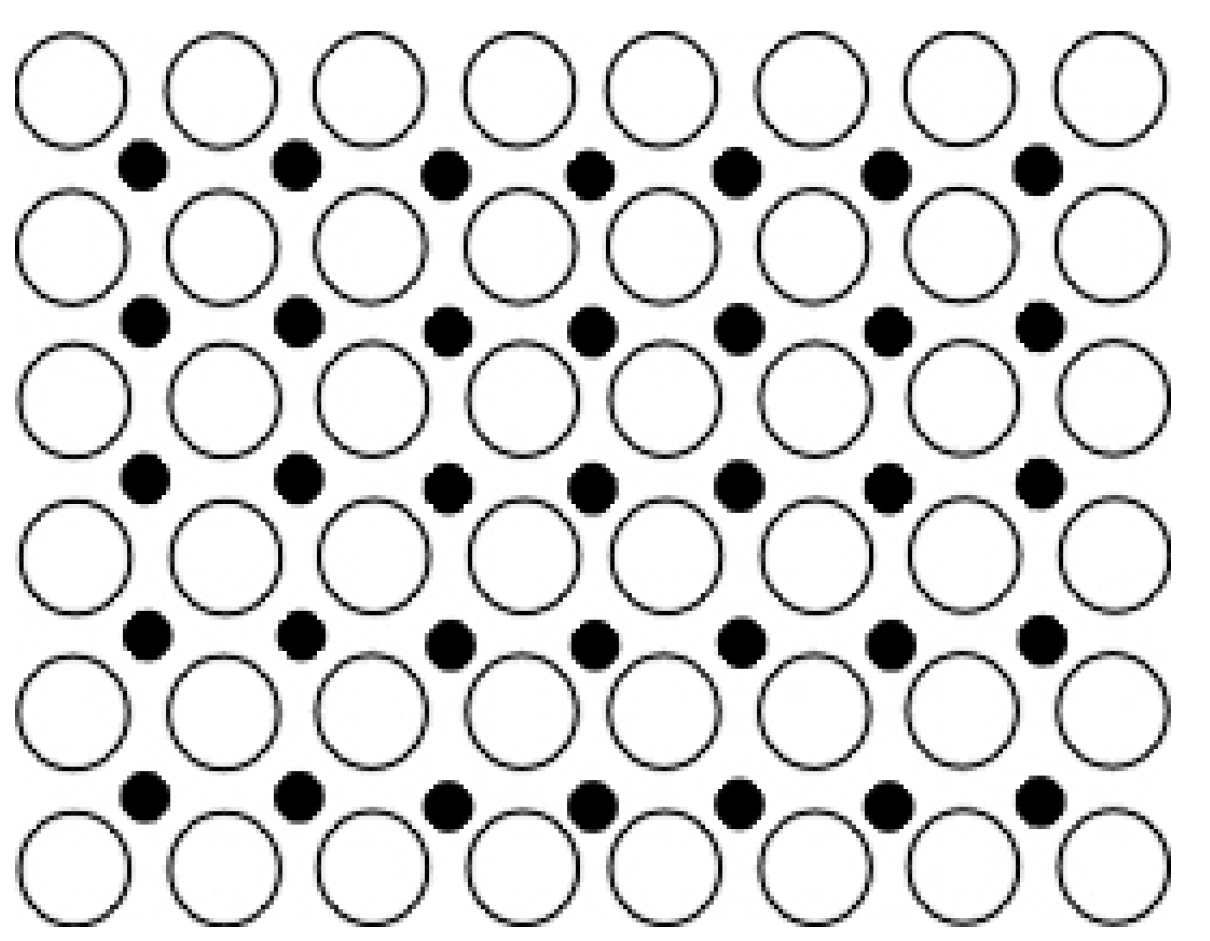
\includegraphics[width=0.75\linewidth]{images/3_Ein_2.png}
		\caption{Kristallit geregelt eingelagert}
	\end{subfigure}
	\begin{subfigure}{0.32\linewidth}
		\centering
		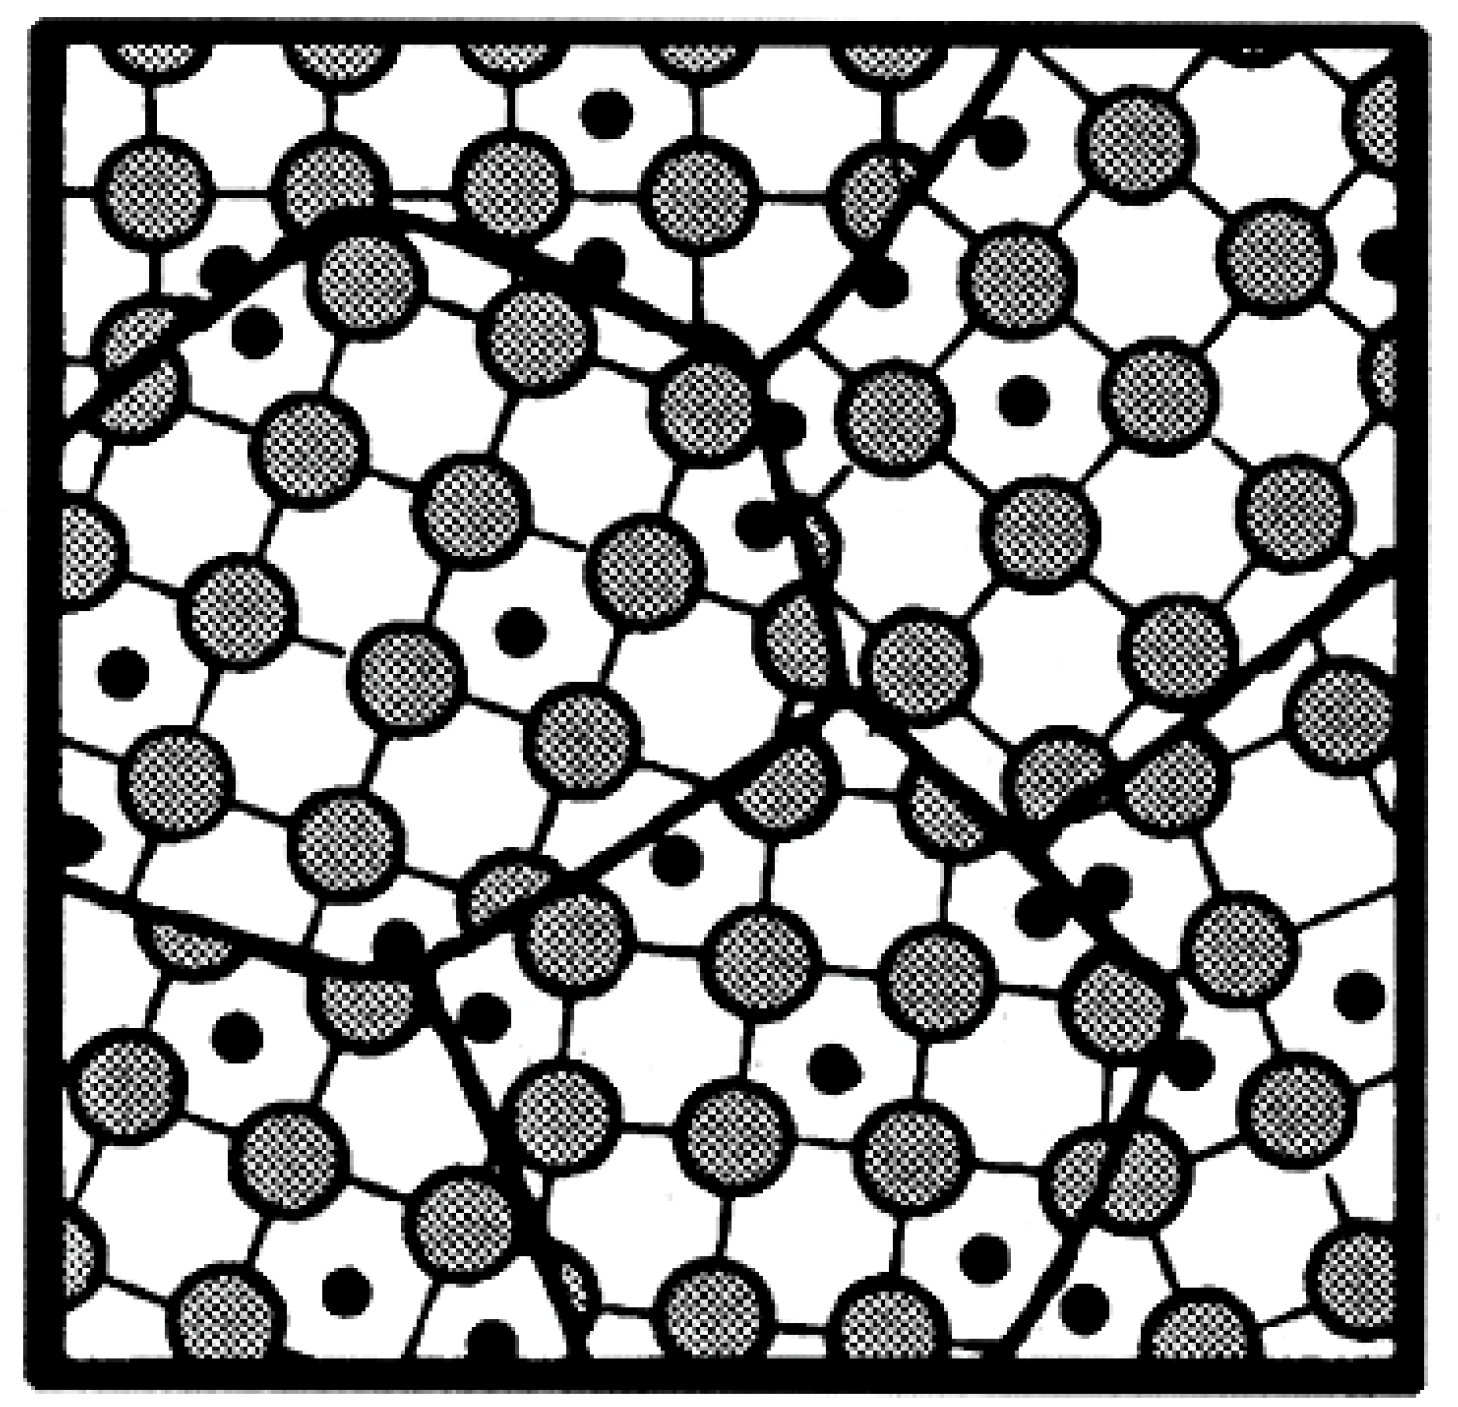
\includegraphics[width=0.75\linewidth]{images/3_Ein_3.png}
		\caption{Aufbau einer ungeregelten Einlagerungslegierung}
	\end{subfigure}
\end{figure}

\subsection{Energiebänder-Modell}
Überlappung von $N$ Atomorbitalen (AO) führt zu $N$ Molekülorbitalen (MO). Wenn $N$ sehr gross $\Rightarrow$ Bänder aus MO $\Rightarrow$ elektrisch leitend.
\begin{itemize}
	\item Metalle: leeres Leitungsband überlappt mit (teilweise) gefülltem Valenzband
	\item Isolatoren: Grosse verbotene Zone zwischen Valenzband und Leitungsband
	\item Eigenhalbleiter: Kleine verbotene Zone
\end{itemize}

\begin{figure}[htbp]
	\centering
	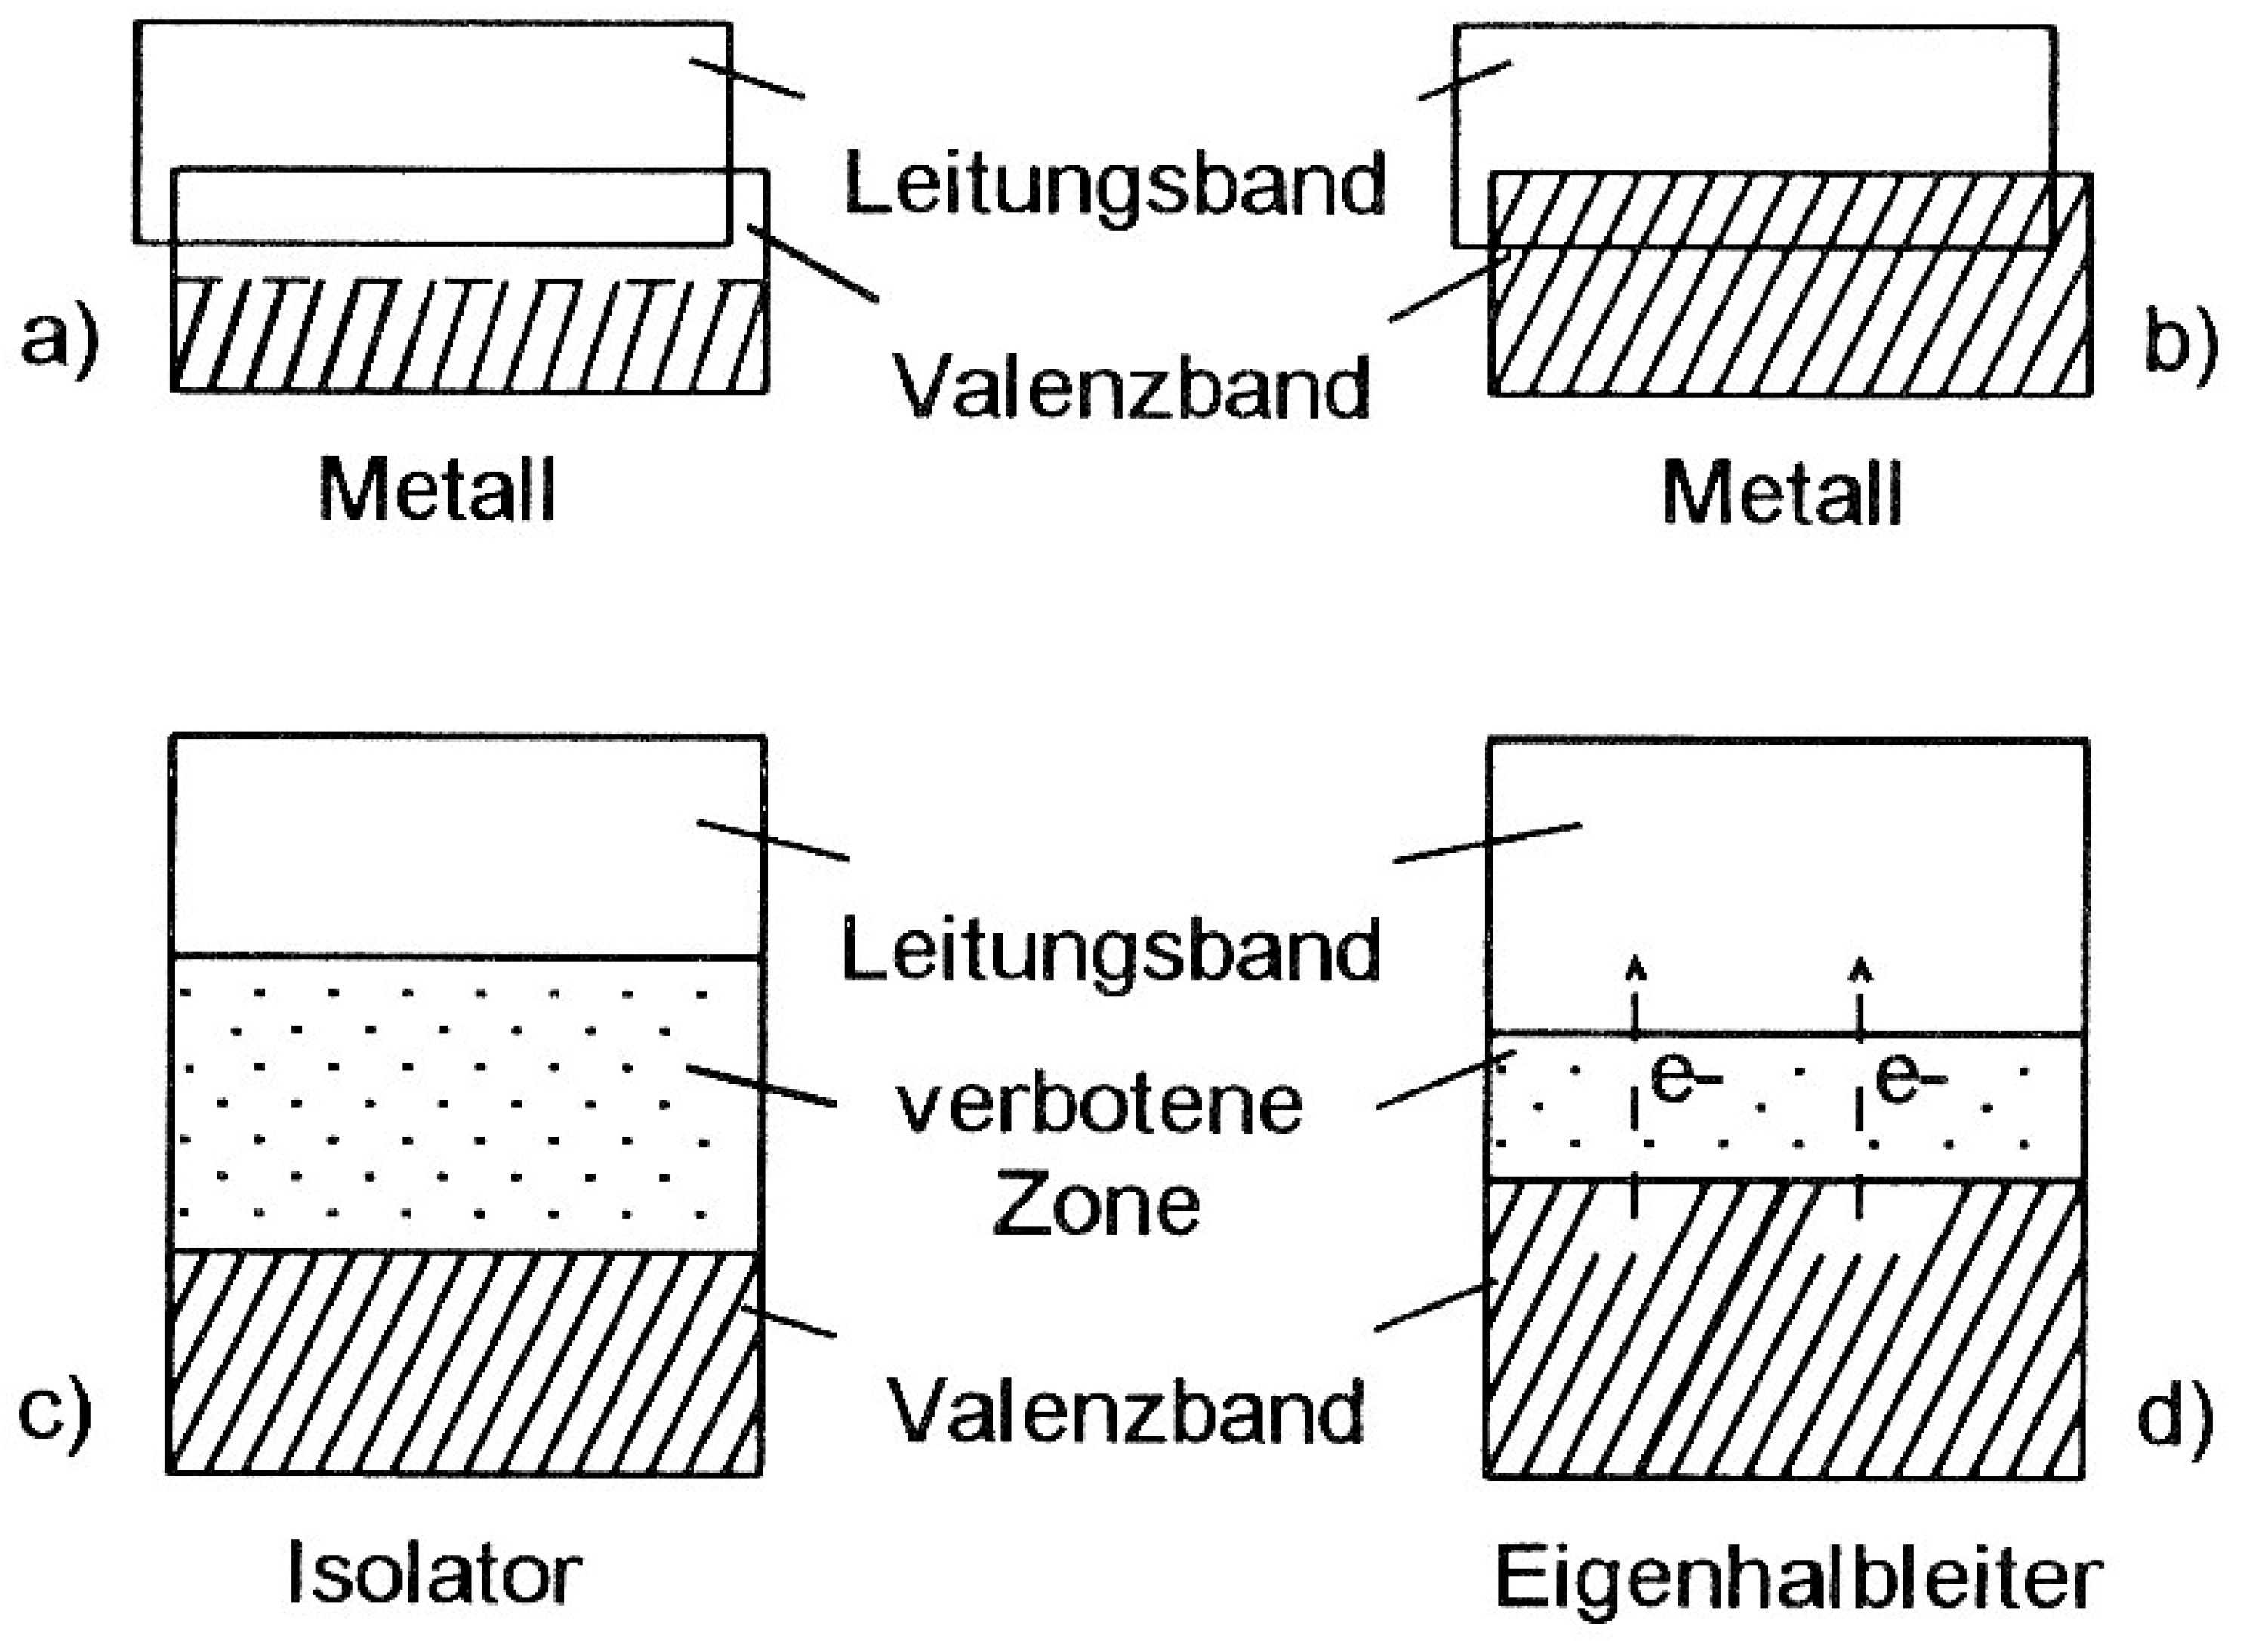
\includegraphics[width=0.9\linewidth, height=0.5\linewidth]{images/3_Energieband.png}
\end{figure}

\subsection{Eisen}
\begin{figure}[h!]
	\centering
	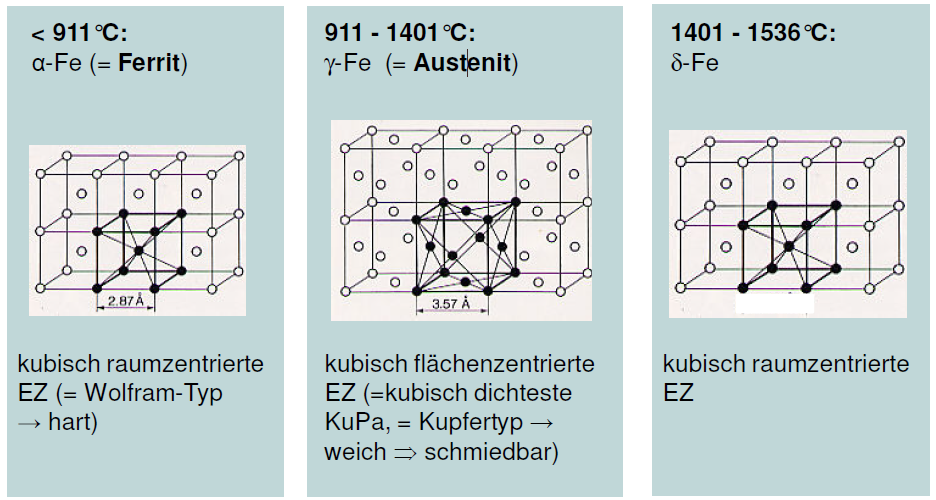
\includegraphics[width=0.9\linewidth]{images/3_Aufbau_Eisen.png}
\end{figure}
